Eine Kugel von \mBO\ wird \hBO\ über dem oberen Ende einer senkrecht stehenden Feder (Federkonstante \kBO) losgelassen. Sie fällt auf die Feder und drückt sie bis zum tiefsten Punkt um $s = \sBP{-2}{3}$ zusammen. Zustand (1): Loslassen, (2): Kugel berührt die Feder, (3): tiefster Punkt. Luftwiderstand und die Masse der Feder sind vernachlässigbar.
\begin{center}
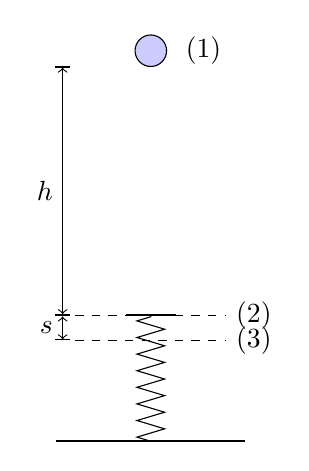
\begin{tikzpicture}[scale=0.8]
 \draw[thick] (-1.5,0) -- (1.5,0);
 \draw[decorate, decoration={zigzag, segment length=6, amplitude=5}] (0,0) -- (0,2);
 \draw[thick] (-0.4,2) -- (0.4,2);
 \draw[dashed] (-1.2,2) -- (1.2,2);
 \draw[dashed] (-1.2,1.6) -- (1.2,1.6);
 \draw[fill=blue!20] (0,6.2) circle (0.25);
 \node[right] at (0.4,6.2) {(1)};
 \node[right] at (1.2,2) {(2)};
 \node[right] at (1.2,1.6) {(3)};
 \draw[|<->|] (-1.4,2) -- (-1.4,5.95) node[midway, left] {$h$};
 \draw[|<->|] (-1.4,1.6) -- (-1.4,2) node[midway, left] {$s$};
\end{tikzpicture}
\end{center}
Eine Schülerin wählt den tiefsten Punkt (3) als Nullniveau der Lageenergie, rechnet mit \gO\ und füllt diese Energietabelle aus:
\begin{center}
\begin{tabular}{lccc}
 & $E_\mathrm{pot}$ & $E_\mathrm{kin}$ & $E_\mathrm{el}$ \\ \hline
 (1) Loslassen & \EwP{0}{3} & \SI{0}{\joule} & \SI{0}{\joule} \\
 (2) Kugel berührt die Feder & \EbP{0}{3} & \EwP{0}{3} & \SI{0}{\joule} \\
 (3) tiefster Punkt & \SI{0}{\joule} & \SI{0}{\joule} & \EcP{0}{3}
\end{tabular}
\end{center}

\begin{abcliste}
\abc
Ein Eintrag der Tabelle ist falsch. Welcher? Was hat die Schülerin falsch gemacht, und was wäre richtig?

\abc
\DuSie{Zeige}{Zeigen Sie} mit der Gesamtenergie, dass die Tabelle so nicht stimmen kann, und dass sie mit dem korrigierten Eintrag stimmt.

\abc
Wie schnell ist die Kugel in (2)?
\end{abcliste}
